\documentclass[12pt]{article}
\usepackage[all, stdclass]{lix}
\usepackage{graphicx}
\usepackage{svg}
\usepackage{url}
\svgsetup{
  inkscapepath=assets/,  % Path to the directory containing your SVG files
  svgpath=assets/        % Path to the directory containing your SVG files
}
\usepackage{float}
\usepackage{hyperref}
\usepackage{times}
\usepackage{amsmath}
\usepackage{caption}
\usepackage{subcaption}
\usepackage{circuitikz}
\usepackage{pgfplots}
\usepackage{pgfplotstable}
\usepackage{tikz}
\usepackage{tikzscale}
%----------EDIT COVER INFO HERE -----------------%

\def \LOGOPATH {assets/birzeit-logo.png}
\def \DEPARTEMENT {Department of Electrical \& Computer Engineering}
\def \COURSENUM {ENEE4113}
\def \COURSENAME {Communications Laboratory}
\def \REPORTTITLE {Pulse Code Modulation (Part 2)}
\def \STUDENTNAME {Mohammad Abu-Shelbaia}
\def \PARTNERAN {Yazan Shrouf}
\def \PARTNERAID {1190145}
\def \PARTNERBN {Taher Hasan}
\def \PARTNERBID {1191740}
\def \STUDENTID {1200198}
\def \INSTRUCTOR {Dr. Ibrahim Nemer}
\def \ASSISTANT {Eng. Mohammad Al-Battat}
\def \REPORTNUM {8}

\begin{document}
\pagenumbering{Roman}

\begin{titlepage}
    \vfill
    \begin{center}
        \includegraphics[width=0.7\textwidth]{\LOGOPATH} \\
        \hfill \\
        \Large{\DEPARTEMENT} \\
        \Large{\COURSENUM\;-\;\COURSENAME} \\
        \vfill
        \textbf{\LARGE{Experiment \#\REPORTNUM}} \\
        \textbf{\LARGE{\REPORTTITLE}}
    \end{center}
    \vfill
    \begin{flushleft}
        \Large{\textbf{Prepared by:}\\ \STUDENTNAME\quad\STUDENTID} \\
        \Large{\textbf{Partners:}\\ 
        \begin{tabular}{@{}l@{\quad}l}
            \PARTNERAN & \PARTNERAID \\
            \PARTNERBN & \PARTNERBID \\
        \end{tabular}} \\
        \Large{\textbf{Instructor:} \INSTRUCTOR} \\
        \Large{\textbf{Assistant:} \ASSISTANT} \\
        \Large{\textbf{Section:} 4}\\
        \LARGE{\textbf{ }}\\
        \LARGE{\textbf{ }}\\
        \LARGE{\textbf{ }}\\
        \Large{\textbf{Date:} \today}\\
    \end{flushleft}
    \vfill
\end{titlepage}

\clearpage
% --------------- ABSTRACT ------------------%
% ---- TABLES --------------------------------%
{
\centering
\section*{Abstract}
In this experiment, we are going to study the process of pulse code modulation (PCM), and the difference in pulse code modulation (DPCM). We are also going to study the effect of quantization noise on the signal.
\clearpage
}

%--------------- TABLES --------------------------------%
\tableofcontents
\clearpage
\setlength{\parskip}{\baselineskip}%
\listoffigures
\clearpage
\pagenumbering{arabic}
%-------------- CONTENT ---------------------%
\h{Theory}
The process of pulse code modulation (PCM) is the process of sampling, quantization, and encoding. 
\hh{Sampling (PAM)}
Sampling is the process of converting a continuous-time signal into a discrete-time signal. In this experiment, we discuss two types of sampling which are natural sampling and flat-top sampling. 
\hhh{Natural Sampling}
In natural sampling, we multiply the message signal by a train of impulses, and the result is a sampled signal as shown below:
\begin{figure}[H]
    \centering
    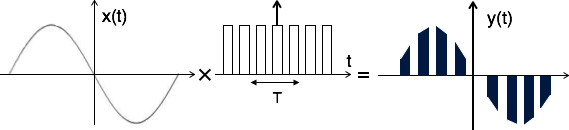
\includegraphics[width=0.5\textwidth]{assets/natural_sampling.png}
    \caption{Natural Sampling}
    \label{fig:1}
    \cite{tutorialspoint}
\end{figure}

\hhh{Flat-Top Sampling}
In flat-top sampling, we multiply the message signal by a train of impulses, but the impulses are not impulses anymore, they are flat-tops, and the result is a sampled signal as shown below:
\begin{figure}[H]
    \centering
    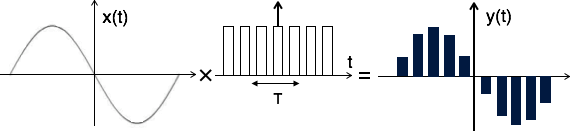
\includegraphics[width=0.5\textwidth]{assets/flat_top_sampling.png}
    \caption{Flat-Top Sampling}
    \label{fig:2}
    \cite{tutorialspoint}
\end{figure}
\hh{Quantization}
Quantization is the process of converting a continuous-valued signal into a discrete-valued signal. In this experiment, we discuss two types of quantization which are linear quantization and non-linear quantization.
In linear quantization, we divide the range of the signal into equal portions and assign a value to each portion.
In non-linear quantization, we divide the range of the signal into portions that are not equal and assign a value to each portion.

\hh{Encoding}
Encoding is the process of converting a discrete-valued signal into a digital signal, There are a lot of encoding methods but the important thing in encoding is the number of bits used to encode the signal which is the resolution of the signal, the higher the resolution the better the signal is encoded, but the higher the resolution the more bandwidth and storage space is needed.

\hh{Difference Pulse Code Modulation (DPCM)}
DPCM is a more efficient method of encoding the signal, it uses the sample of the previous signal to predict the sample of the current signal, and the noise is the difference between the predicted sample and the actual sample. The DPCM is shown in the figure below:
\begin{figure}[H]
    \centering
    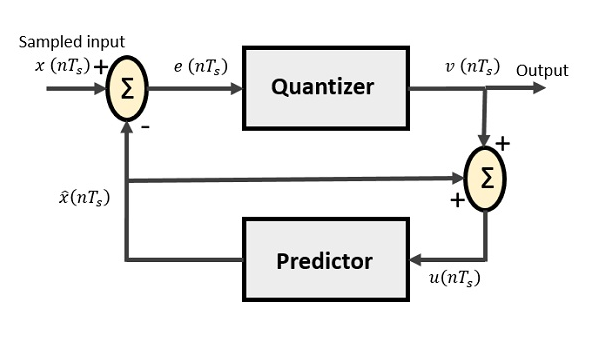
\includegraphics[width=0.5\textwidth]{assets/dpcm_transmitter.jpg}
    \caption{Difference Pulse Code Modulation (DPCM)}
    \label{fig:3}
    \cite{tutorialspoint2}
\end{figure}
\clearpage
\h{Procedure and Data Analysis}
\begin{figure}[H]
    \centering
    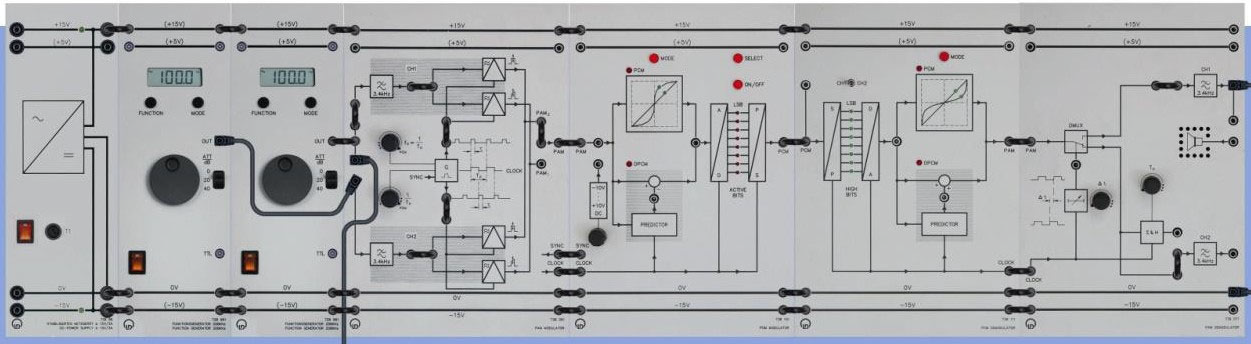
\includegraphics[width=\textwidth]{assets/main/2023-08-26-21-51-59.png}
    \caption{Circuit Diagram}
    \cite{manual}
    \label{fig:1}
\end{figure}
The circuit in figure \ref{fig:1} is the blocks that we used in this experiment, the first block from the left is the power source, the two following blocks are function generators, then comes the PAM modulator, then the PCM modulator, then the PCM demodulator, and finally the PAM demodulator.
\hh{PCM with TDM}
In this part, we set up two signals the first one is a sine wave:
\begin{equation}
    V_{1} = 10 \sin(2\pi (300) t)
\end{equation}
The second one is a triangle wave:
\begin{equation}
    V_{2} = 5 \wedge(2\pi (200) t)
\end{equation}
for the PAM modulator, we set the duty-cycle knob to the maximum, and the sampling frequency knob to the minimum. We also set the encoding bits to the maximum and connected all the modules, finally, we plotted the input signals with the demodulated signals and the results were as follows:
\begin{figure}[H]
    \centering
    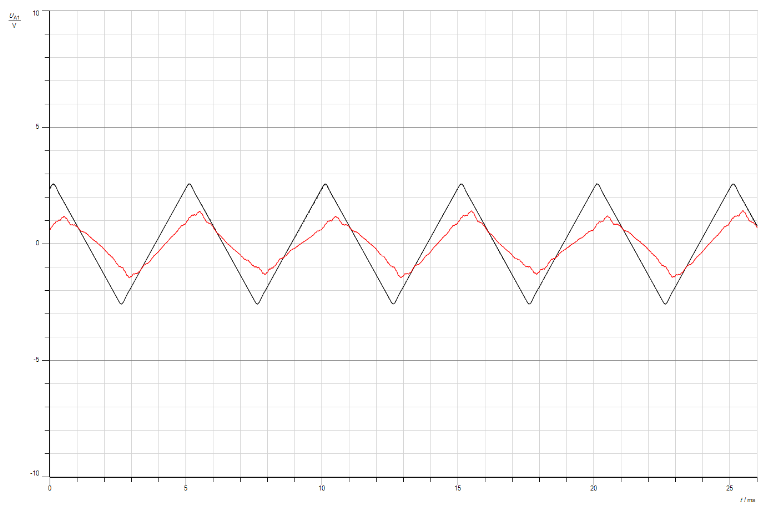
\includegraphics[width=0.49\textwidth]{assets//main/2023-08-26-22-19-56.png}
    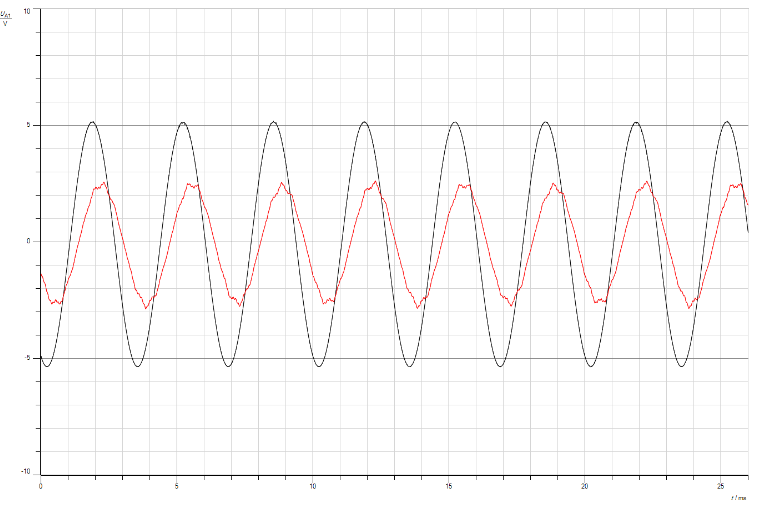
\includegraphics[width=0.49\textwidth]{assets/main/2023-08-26-22-20-30.png}
    \caption{PAM Modulator and Demodulator}
    \label{fig:2}
\end{figure}
The results in (Figure \ref{fig:2}) show that the PAM modulator and demodulator are working as expected, and the signals were recovered correctly but its not the same as the original signal in terms of amplitude and smoothness due to the sampling and quantization process, but even though the signal is still recognizable.
\hh{Quantaization Noise}
In this part, we intend to study the effect of quantization noise on the signal by plotting the signal with a different number of bits. 
\hhh{Triangle Wave with Linear Quantaization}
First, we initially connected both PAM modulator channels to the function generator signal:
\begin{equation}
    V_{1} = 12 \wedge(2\pi (30) t)
\end{equation}
with 8-bit/5-bit linear quantization, and we plotted the message signal and the digitized signal (PCM Demodulator output) and the results were as follows:
\begin{figure}[H]
    \centering
    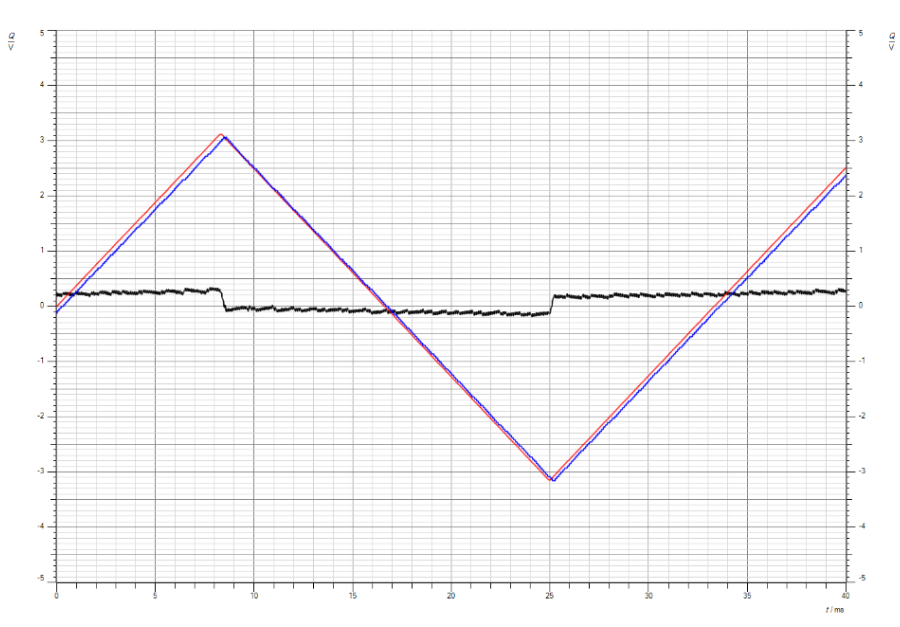
\includegraphics[width=0.49\textwidth]{assets/main/2023-08-26-22-30-20.png}
    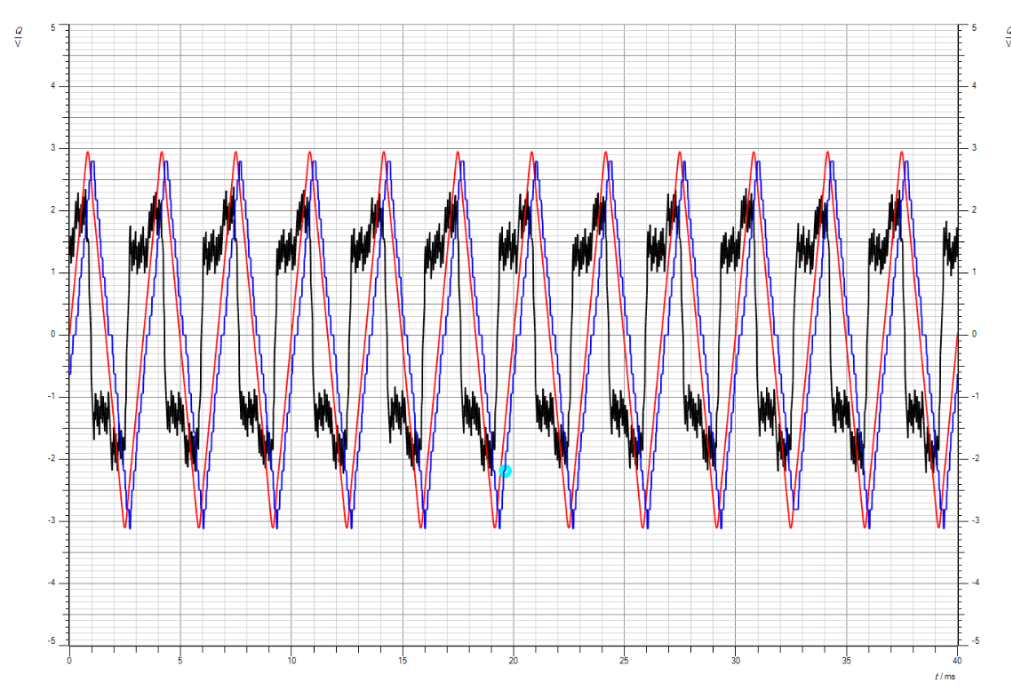
\includegraphics[width=0.49\textwidth]{assets/main/2023-08-26-22-36-58.png}
    \caption{8-bit/5-bit Linear Quantaization}
    \label{fig:3}
\end{figure}
We saw that there are three waveforms while we are measuring only two, The third one is the noise which is the difference between the original signal and the digitized signal, and we can see that the noise is very small and almost negligible for the 8-bit encoding. Then we repeated the same procedure but with 5-bit encoding, we saw that the noise is much larger than the 8-bit encoding and it is not negligible anymore. We should've also studied the effect of changing the resolution without changing the frequency but we didn't notice that until we finished the experiment.
\hhh{Sine Wave with Non-Linear Quantaization}
In this part, we connected the PAM modulator to the function generator signal:
\begin{equation}
    V_{1} = 12 \sin(2\pi (30) t)
\end{equation}
with 8-bit/5-bit non-linear quantization, and we plotted the message signal and the digitized signal (PCM Demodulator output) and the results were as follows:
\begin{figure}[H]
    \centering
    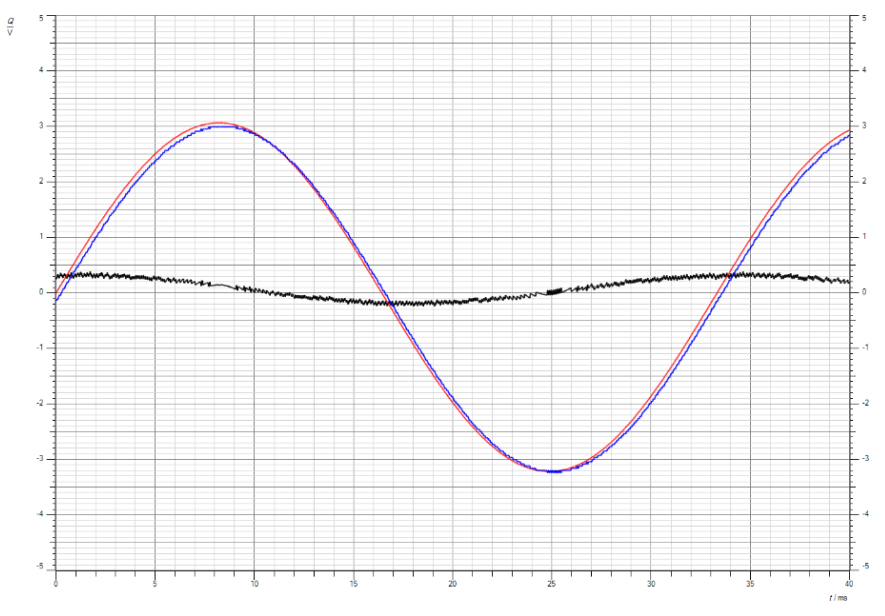
\includegraphics[width=0.49\textwidth]{assets/main/2023-08-26-22-44-32.png}
    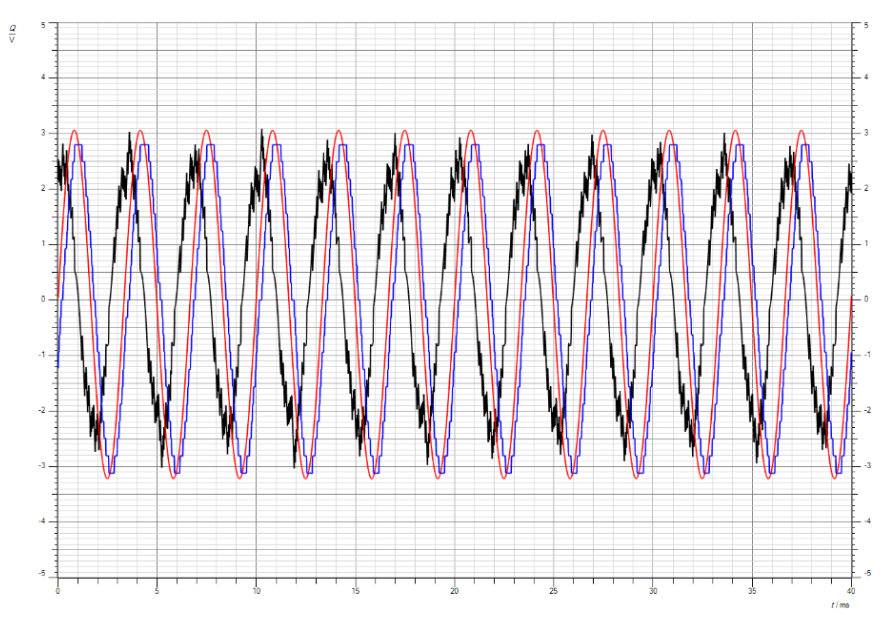
\includegraphics[width=0.49\textwidth]{assets/main/2023-08-26-22-44-52.png}
    \caption{8-bit/5-bit Non-Linear Quantaization}
    \label{fig:4}
\end{figure}
We saw that the noise is still negligible for the 8-bit encoding, and it is a bit larger than the linear quantization noise, and for the 5-bit encoding the noise is much larger than the 8-bit encoding and it is not negligible anymore. We of course should've also studied the effect of changing the resolution without changing the frequency but as mentioned before we didn't notice that until we finished the experiment.
\hh{Difference Pulse Code Modulation (DPCM)}
After synchronizing the process, we plotted the message signal with five different signals which are the predictor of the DPCM Modulator, the output of the DPCM Modulator, the input of the DPCM Demodulator, the predictor of the DPCM Demodulator, and the output of the DPCM Demodulator, and the results were as follows for 8-bit quantization:
\begin{figure}[H]
    \begin{subfigure}[b]{0.49\textwidth}
        \centering
        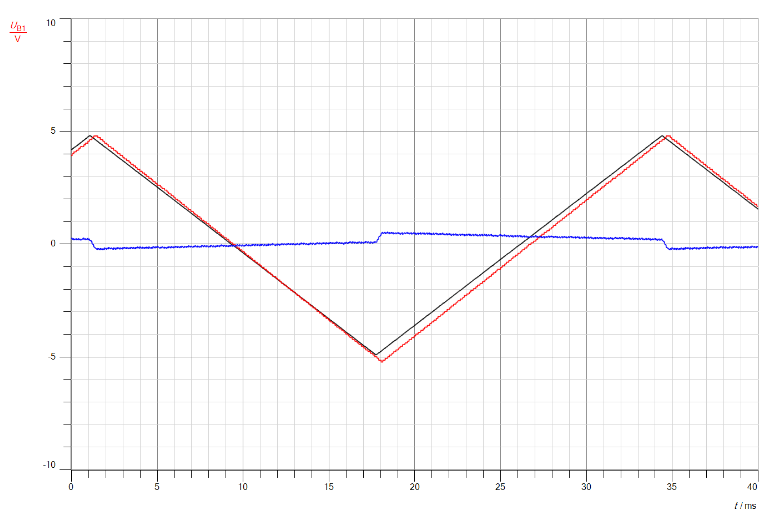
\includegraphics[width=\textwidth]{assets/main/2023-08-26-22-58-44.png}
        \caption{DPCM Predictor}
    \end{subfigure}
    \begin{subfigure}[b]{0.49\textwidth}
        \centering
        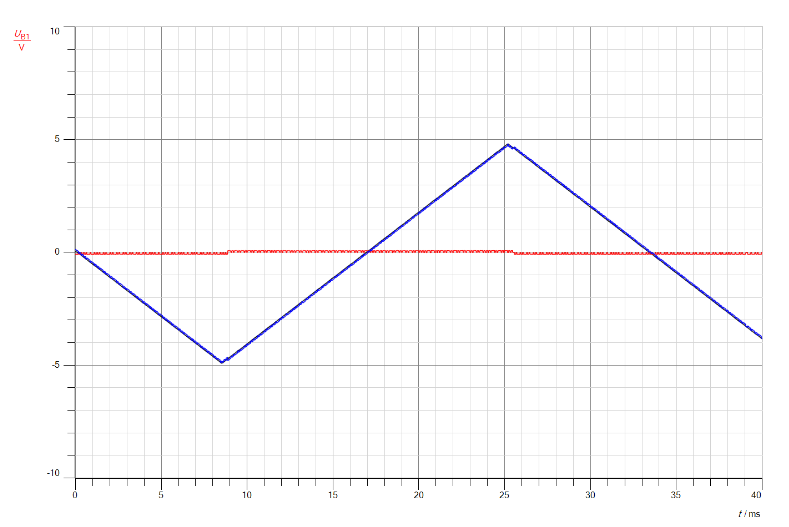
\includegraphics[width=\textwidth]{assets/main/2023-08-26-23-04-49.png}
        \caption{DPCM Output}
    \end{subfigure}
    \caption{8-bit DPCM Modulator}
\end{figure}

\begin{figure}[H]
    \begin{subfigure}[b]{0.32\textwidth}
        \centering
        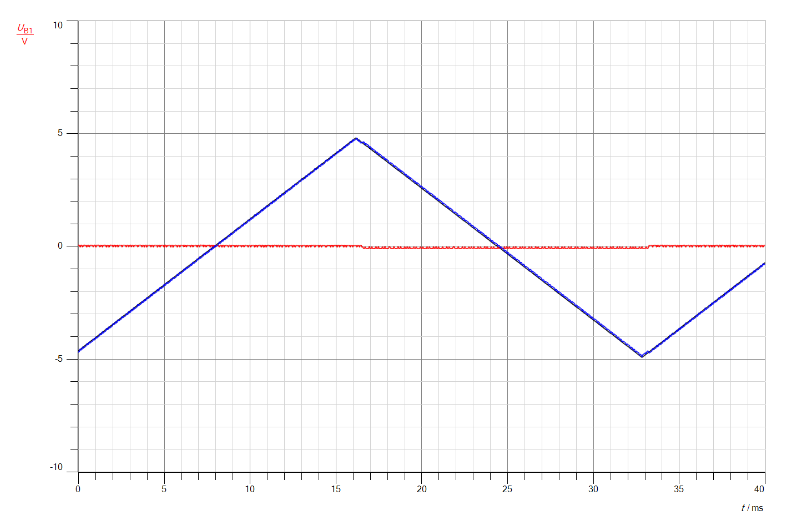
\includegraphics[width=\textwidth]{assets/main/2023-08-26-23-07-23.png}
        \caption{DPCM Input}
    \end{subfigure}
    \begin{subfigure}[b]{0.32\textwidth}
        \centering
        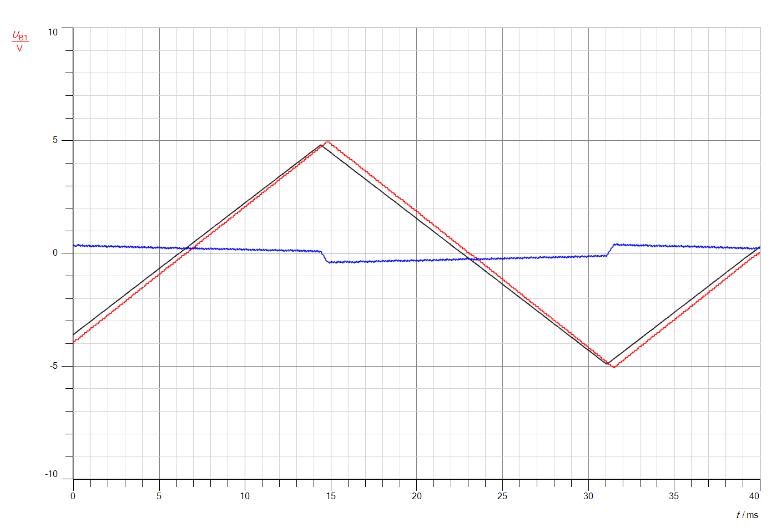
\includegraphics[width=\textwidth]{assets/main/2023-08-26-23-07-45.png}
        \caption{DPCM Predictor}
    \end{subfigure}
    \begin{subfigure}[b]{0.32\textwidth}
        \centering
        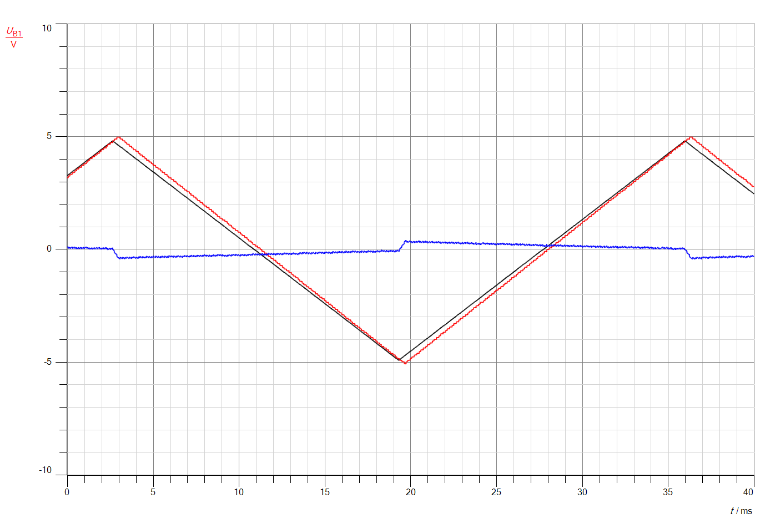
\includegraphics[width=\textwidth]{assets/main/2023-08-26-23-10-45.png}
        \caption{DPCM  Output}
    \end{subfigure}
    \caption{8-bit DPCM Demodulator}
\end{figure}

We notice that the DPCM Modulator has a little difference from the message signal, This difference gets corrected and at the Modulator output we get the same message signal, and the same thing happens at the Demodulator input, but at the Demodulator output we get a little difference from the message signal, and this difference is the quantization noise. We repeated the same procedure but with 4-bit quantization and the results were as follows:
\begin{figure}[H]
    \begin{subfigure}[b]{0.49\textwidth}
        \centering
        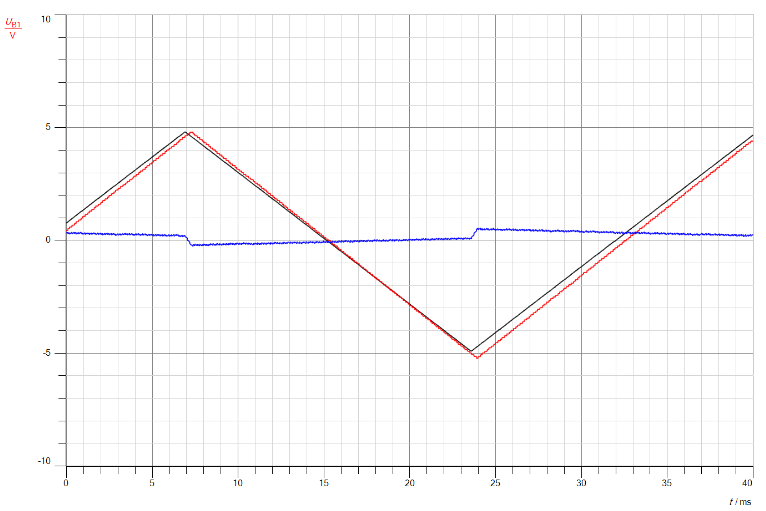
\includegraphics[width=\textwidth]{assets/main/2023-08-26-23-15-09.png}
        \caption{DPCM Predictor}
    \end{subfigure}
    \begin{subfigure}[b]{0.49\textwidth}
        \centering
        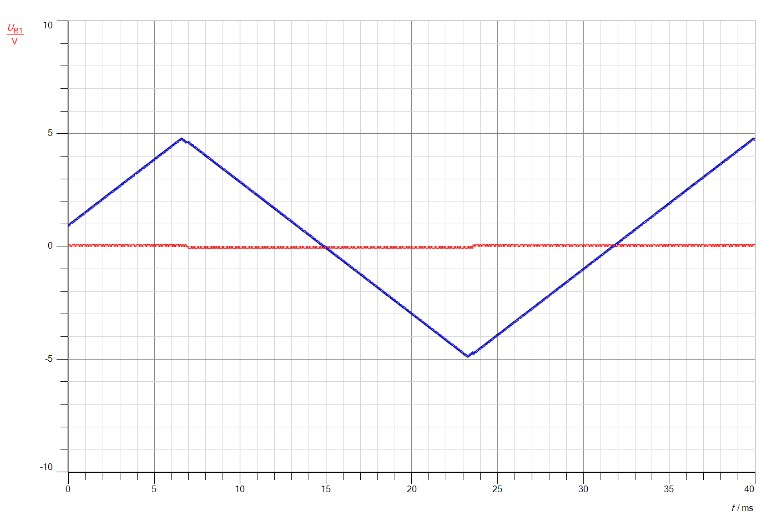
\includegraphics[width=\textwidth]{assets/main/2023-08-26-23-15-26.png}
        \caption{DPCM Output}
    \end{subfigure}
    \caption{4-bit DPCM Modulator}
\end{figure}

\begin{figure}[H]
    \begin{subfigure}[b]{0.32\textwidth}
        \centering
        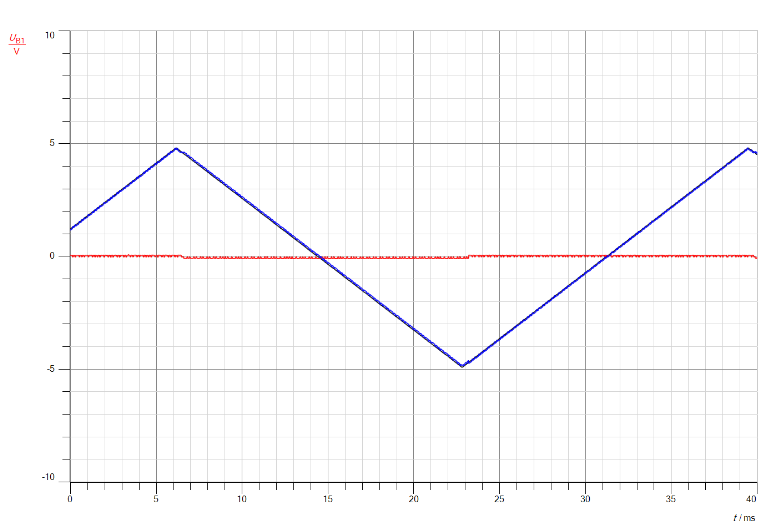
\includegraphics[width=\textwidth]{assets/main/2023-08-26-23-15-46.png}
        \caption{DPCM Input}
    \end{subfigure}
    \begin{subfigure}[b]{0.32\textwidth}
        \centering
        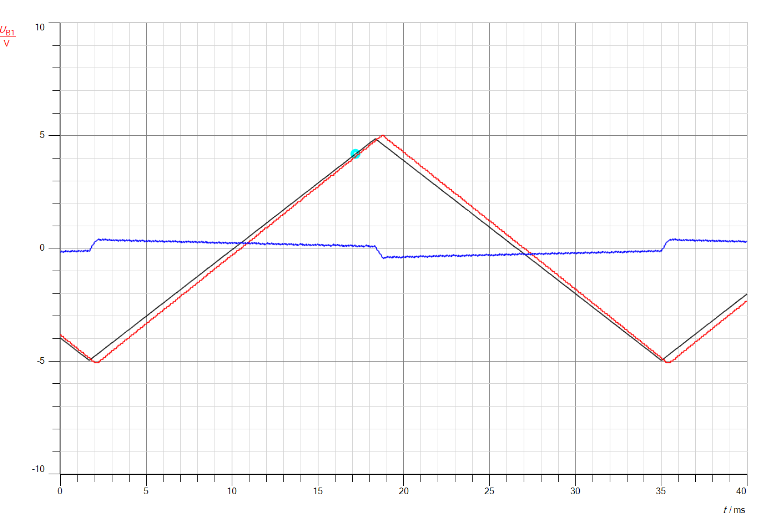
\includegraphics[width=\textwidth]{assets/main/2023-08-26-23-16-03.png}
        \caption{DPCM Predictor}
    \end{subfigure}
    \begin{subfigure}[b]{0.32\textwidth}
        \centering
        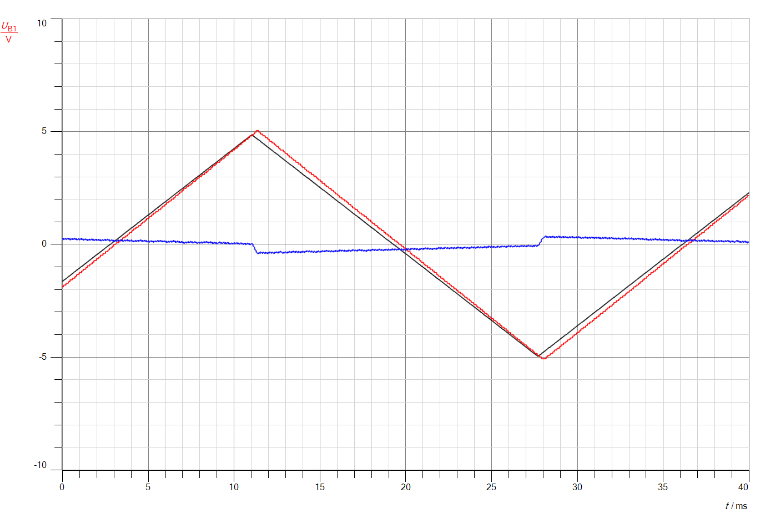
\includegraphics[width=\textwidth]{assets/main/2023-08-26-23-16-27.png}
        \caption{DPCM Output}
    \end{subfigure}
    \caption{4-bit DPCM Demodulator}
\end{figure}
We notice that the modulation process is the same as the 8-bit quantization and the demodulation process is also the same as the 8-bit quantization, there is almost no visible difference between the 8-bit and 4-bit. This concludes that the DPCM is a very efficient method of encoding the signal since it could use fewer bits to encode the signal and still get the same results as the 8-bit quantization, which lets us save bandwidth and storage space.
\clearpage
\h{Conclusion}
In conclusion, we learned the process of pulse code modulation (PCM), and the difference pulse code modulation (DPCM). We also learned the effect of quantization noise on the signal, and we learned that the DPCM is a very efficient method of encoding the signal since it could use fewer bits to encode the signal and still get the same results as the 8-bit quantization, which lets us save bandwidth and storage space.
\clearpage
\bibliographystyle{IEEEtran}
\bibliography{cites}
\clearpage
\end{document}
